% Intended LaTeX compiler: xelatex
\documentclass[10pt, svgnames]{beamer}
\usepackage{graphicx}
\usepackage{longtable}
\usepackage{wrapfig}
\usepackage{rotating}
\usepackage[normalem]{ulem}
\usepackage{amsmath}
\usepackage{amssymb}
\usepackage{capt-of}
\usepackage{hyperref}
\usetheme{focus}
\author{Sappinandana Akamphon}
\date{\today}
\title{Analysis of Members under Bending}
\subtitle{ME 210: Mechanics of Materials}
\usepackage{booktabs}
\usepackage{pgfplots}
\pgfplotsset{compat=1.18}
\institute{Department of Mechanical Engineering, TSE}
\date{}
\usetikzlibrary{patterns,shapes,arrows}
\AtBeginSection[]{\begin{frame}{Outline}\tableofcontents[currentsection]\end{frame}}
\hypersetup{
 pdfauthor={Sappinandana Akamphon},
 pdftitle={Analysis of Members under Bending},
 pdfkeywords={},
 pdfsubject={},
 pdfcreator={Emacs 30.0.50 (Org mode 9.6)}, 
 pdflang={English}}
\usepackage{biblatex}

\begin{document}


\begin{frame}[label={sec:org39d9269}]{\{\}}
\maketitle
\end{frame}

\section{Overview of Bending}
\label{overview-of-bending}
\begin{frame}[label={sec:org8eee984}]{What is Bending?}
\begin{itemize}
\item Curving of a long, slender member under moment or force

\item Caused by bending moment: moment whose direction is perpendicular to member axis
\end{itemize}
\end{frame}

\begin{frame}[label={sec:org61fcb47}]{Sign Convention}
\begin{itemize}
\item Shear force and bending moment follow these sign conventions
\end{itemize}

\begin{center}
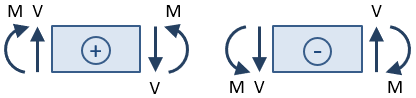
\includegraphics[width=.9\linewidth]{pictures/sign-convention.png}
\end{center}
\end{frame}

\begin{frame}[label={sec:org65b9c93}]{Beam Curvature}
\begin{itemize}
\item In bending, beam curves in response to bending moment
\end{itemize}

\begin{columns}
\begin{column}{0.6\columnwidth}
\begin{center}
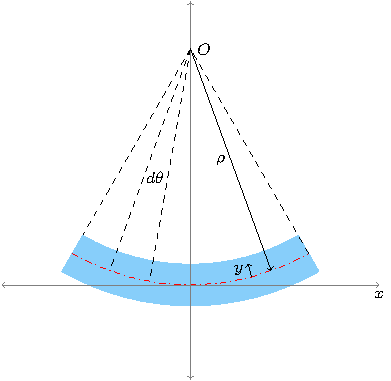
\includegraphics[width=.9\linewidth]{pictures/beam-curvature.pdf}
\end{center}
\end{column}

\begin{column}{0.4\columnwidth}
\[\kappa = \frac{1}{\rho}\]

\begin{itemize}
\item Assume beam is thin compared to its curvature (\(h \ll \rho\))

\item This way, curvature of beam is constant throughout thickness
\end{itemize}
\end{column}
\end{columns}
\end{frame}

\begin{frame}[label={sec:org92212b7}]{Longitudinal Strain in Beam}
\begin{columns}
\begin{column}{0.6\columnwidth}
\begin{center}
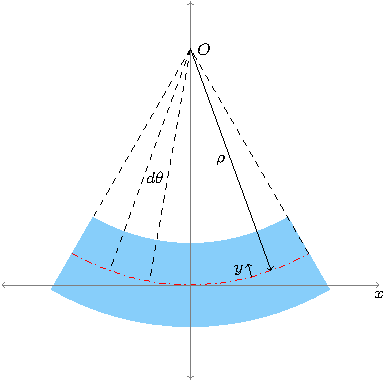
\includegraphics[width=.9\linewidth]{pictures/strain-in-beam.pdf}
\end{center}
\end{column}

\begin{column}{0.4\columnwidth}
\begin{itemize}
\item Longitudinal strain vary across thickness

\[\varepsilon_x = - \frac{y}{R} = -\kappa y\]

\item No strain where \(y\) = 0 \(\rightarrow\) \emph{Neutral Axis}

\item So where is this \(R\)?
\end{itemize}
\end{column}
\end{columns}
\end{frame}

\begin{frame}[label={sec:org1dcac39}]{Stress in Beam Bending}
\begin{itemize}
\item Again, assuming linear elastic deformation
\end{itemize}

\[\sigma_x = E \varepsilon_x = - \frac{Ey}{R}\]

\begin{itemize}
\item With this, we can now find \(R\)
\end{itemize}
\end{frame}

\begin{frame}[label={sec:org07b7d44}]{In Search of \(R\)}
\begin{itemize}
\item Any arbitrary cross section must be at rest
\end{itemize}

\[\int_A \sigma_x dA = - \int_A E \kappa y dA = 0\]

\begin{itemize}
\item For uniform material and \emph{thin} beam (\(\kappa\) is constant)
\end{itemize}

\[\int_A y dA = 0\]

\begin{itemize}
\item What does this equation remind you of?
\end{itemize}
\end{frame}

\begin{frame}[label={sec:orge38fdc3}]{Example: Neutral Axis of a Triangular Cross Section}
\begin{columns}
\begin{column}{0.3\columnwidth}
\begin{center}
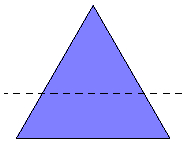
\includegraphics[width=\textwidth]{./pictures/triangular-section-axis.pdf}
\end{center}
\end{column}

\begin{column}{0.6\columnwidth}
\[\int_A y dA = 0\]

cut triangle into thin horizontal strips. strip
width \(w\) is a function of \(y\), so

\begin{align*}
        w = b \left( 1 - \frac{y}{h} \right)
\end{align*}
\end{column}
\end{columns}
\end{frame}

\begin{frame}[label={sec:orga4ed3cb}]{Solution}
\begin{columns}
\begin{column}{0.3\columnwidth}
\begin{center}
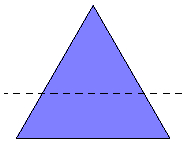
\includegraphics[width=.9\linewidth]{./pictures/triangular-section-axis.pdf}
\end{center}
\end{column}

\begin{column}{0.6\columnwidth}
\begin{align*}
  0 &= \int_{0}^{h} w(y - y_{NA})dy \\
    &= \int_{0}^{h} b \left( 1- \frac{y}{h} \right)(y - y_{NA})dy \\
    &= \frac{b}{h} \int_{0}^{h} (hy - hy_{NA} - y^{2} + yy_{NA})dy \\
    &= \frac{b}{h} \left( h \frac{y^{2}}{2} - hy_{NA}y - \frac{y^{3}}{3} + y_{NA}\frac{y^{2}}{2} \right)_{0}^{h}
\end{align*}

divide through with \(y\) and substitute with \(h\) and 0

\begin{align*}
  0 &= \frac{h^{2}}{2} - hy_{NA} - \frac{h^{2}}{3} + \frac{y_{NA}h}{2} \\
  y_{NA} &= \frac{h}{3}
\end{align*}
\end{column}
\end{columns}
\end{frame}

\section{Moment-Curvature-Stress Relationship}
\label{moment-curvature-stress-relationship}
\begin{frame}[label={sec:org4f8e70f}]{Moment - Curvature Relationship}
\begin{columns}
\begin{column}{0.4\columnwidth}
\[dM = - \sigma_x y dA\]
\[M = - \int_A \sigma_A y dA = \int_A \kappa E y^2 dA\]
\[M = \kappa E I\] \[I = \int_A y^2 dA\]

\[\sigma_x = - E\kappa y\] \[\kappa = - \frac{ \sigma_x }{Ey}\]
\end{column}

\begin{column}{0.6\columnwidth}
\begin{center}
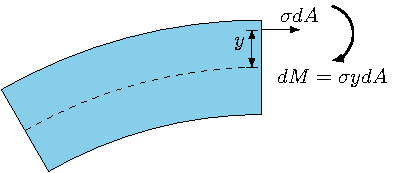
\includegraphics[width=.9\linewidth]{pictures/moment-curvature.pdf}
\end{center}

\begin{gather*}
      \kappa = \frac{M}{EI} \hspace{2cm} \kappa = -\frac{\sigma_{x}}{Ey} \\
      \sigma_{x} = -\frac{My}{I}
\end{gather*}
\end{column}
\end{columns}
\end{frame}

\begin{frame}[label={sec:orgac5c1f6}]{Moment of Inertia, \(I\)}
\begin{align*}
    I = \int_{A} y^{2}dA
\end{align*}

\begin{itemize}
\item Represent resistance of cross section to bending

\item Useful formulae
\end{itemize}

\begin{align*}
  I_{\text{rect}} = \frac{bh^{3}}{12} \\
  I_{\text{circ}}= \frac{\pi R^{4}}{4}
\end{align*}
\end{frame}

\begin{frame}[label={sec:org077aed5}]{Section Modulus \(S\)}
\begin{itemize}
\item Max stress occurs furthest away from \emph{NA}
\end{itemize}

\begin{align*}
  \sigma_1 &= -\frac{Mc_1}{I} = -\frac{M}{S_1} \\
  \sigma_2 &= -\frac{Mc_2}{I} = -\frac{M}{S_2}
\end{align*}

\begin{itemize}
\item Useful in choosing beam sections from catalog
\end{itemize}

\begin{align*}
  S_{1} = \frac{I}{c_{1}} \\
  S_{2} = \frac{I}{c_{2}}
\end{align*}
\end{frame}

\section{Nonuniform Bending}
\label{nonuniform-bending}
\begin{frame}[label={sec:org467eaf4}]{Nonuniform Bending}
\begin{itemize}
\item In \emph{uniform} or \emph{pure} bending, \(M\) is constant along beam length

\begin{itemize}
\item From applying bending moment directly
\end{itemize}

\item Most beams are loaded by lateral forces

\begin{itemize}
\item Gives rise to internal shear forces and stresses
\end{itemize}
\end{itemize}

\[V = \frac{dM}{dx}\]
\end{frame}

\begin{frame}[label={sec:org3c3cb08}]{Transverse Shear Stress in Beam}
\begin{columns}
\begin{column}{0.5\columnwidth}
\begin{center}
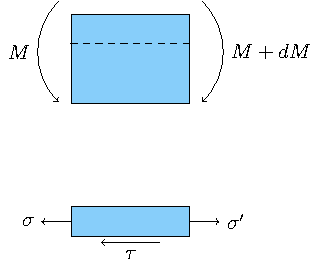
\includegraphics[width=.9\linewidth]{pictures/shear-in-beam.pdf}
\end{center}
\end{column}

\begin{column}{0.5\columnwidth}
\begin{align*}
  \tau t dx &= \int_{A'} \sigma' dA' - \int_{A'} \sigma dA' \\
            &= \int_{A'} \frac{ (M + dM)y }{I} dA' - \int_{A'} \frac{My}{I} dA' \\
            &= \int_{A'} \frac{dMy}{I} dA'
\end{align*}

\begin{align*}
  \tau &= \frac{1}{It} \left( \frac{dM}{dx} \right) \int_{A'} y dA' \\
       &= \frac{VQ}{It}
\end{align*}
\end{column}
\end{columns}
\end{frame}

\begin{frame}[label={sec:org7841ac5}]{What is Q?}
\begin{center}
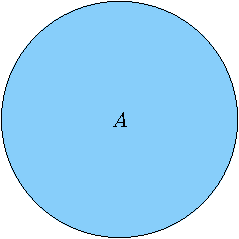
\includegraphics[width=0.3\textwidth]{pictures/first-moment.pdf}
\end{center}

\begin{align*}
    Q &= \text{ first moment of area} \\
      &= \int_{A'} ydA' \neq \int_A ydA \\
      &= A'\bar{y}'
\end{align*}
\end{frame}

\begin{frame}[label={sec:orgfde455d}]{What is Q? (2)}
\begin{center}
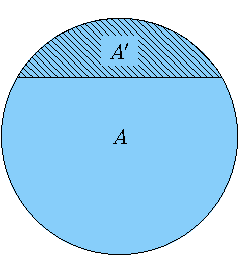
\includegraphics[width=0.3\textwidth]{pictures/first-moment-2.pdf}
\end{center}

\begin{align*}
    Q &= \text{ first moment of area} \\
      &= \int_{A'} ydA' \neq \int_A ydA \\
      &= A'\bar{y}'
\end{align*}
\end{frame}

\begin{frame}[label={sec:orgc9b515d}]{Example: Shear Stress Distribution in Rectangular Beam}
\begin{center}
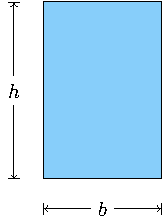
\includegraphics[width=0.2\textwidth]{pictures/shear-stress-example.pdf}
\end{center}

\begin{align*}
  Q(y) &= A^{\prime}\bar{y}^{\prime} \\
       &= \left[ \left( \frac{h}{2} - y \right) b \right] \left[y + \frac{\frac{h}{2} - y}{2} \right] \\
       &= \frac{b}{2} \left( \frac{h^{2}}{4} - y^{2} \right)
\end{align*}
\end{frame}

\begin{frame}[label={sec:orgc63280f}]{Solution}
\begin{align*}
  Q_{\max} &= Q(y = 0) \\
           &= \frac{bh^{2}}{8} \\
  \tau_{\max} &= \frac{VQ}{It} \\
           &= \frac{V \frac{bh^{2}}{8}}{ \frac{bh^{3}}{12} b} \\
           &= \frac{3V}{2bh}  = \frac{3V}{2A}
\end{align*}
\end{frame}

\begin{frame}[label={sec:orga4fe826}]{Example: Maximum shear stress in a circular cross-sectioned beam}
A cantilever beam with length \(L\) and radius \(r\) has a force \(P\)
applied at the middle. Determine the location and magnitude of maximum
shear stress.

\begin{itemize}
\item Maximum shear force in the beam is anywhere from the fixed end to the
middle

\item Maximum shear stress occurs at NA

\item Anywhere along NA from the fixed end to the middle has max shear
stress
\end{itemize}
\end{frame}

\begin{frame}[label={sec:org82f021e}]{Solution}
\begin{itemize}
\item Now, for the magnitude
\end{itemize}

\begin{align*}
  \tau &= \frac{VQ}{Ib} = \frac{P ((\pi/2) r^{2} (4r/3\pi))}{(\pi/4)r^{4}(2r)} \\
       &= \frac{4P}{3 \pi r^{2}} = \frac{4P}{3A}
\end{align*}
\end{frame}

\section{Composite Beam Bending}
\label{composite-beam-bending}
\begin{frame}[label={sec:org7fac777}]{Composite Beam Bending}
\begin{itemize}
\item Two or more materials (\(E_{1} \neq E_{2} \neq \ldots\))

\item Deformation (and strain) remain unchanged
\end{itemize}

\[\varepsilon_x = -\frac{y}{R} = -\kappa y\]

\begin{itemize}
\item But where is the new neutral axis?

\item Since sectional property is no longer uniform \(\rightarrow\) neutral
axis will move
\end{itemize}
\end{frame}

\begin{frame}[label={sec:org0e9b76e}]{Neutral Axis of a Composite Beam}
\begin{columns}
\begin{column}{0.5\columnwidth}
\begin{center}
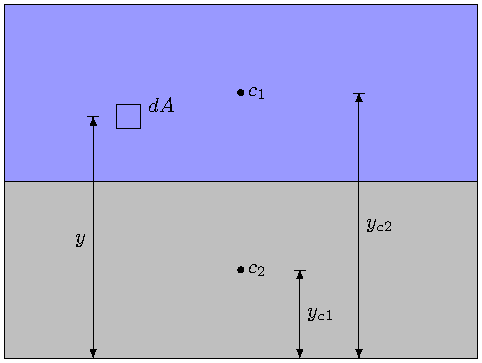
\includegraphics[width=.9\linewidth]{./pictures/na-composite.pdf}
\end{center}
\end{column}

\begin{column}{0.5\columnwidth}
\[\int_{A1} \sigma_{x1} dA + \int_{A2} \sigma_{x2} dA = 0\]
\[- \int_{A1} E_1 \kappa y dA - \int_{A2} E_2 \kappa y dA = 0\]
\[- E_1 \int_{A1} y dA - E_2 \int_{A2} y dA = 0\]
\[E_1 y_{c1} A_1 + E_2 y_{c2} A_2 = 0\]

This works for more than 2 materials as well!
\end{column}
\end{columns}
\end{frame}

\begin{frame}[label={sec:org6972fc6}]{Moment-Curvature for Composite Beams}
\begin{itemize}
\item Same equation applies, only different results
\end{itemize}

\begin{align*}
  M &= - \int_A \sigma y dA \\
    &= -\int_{A1} \sigma_{x1} y dA - \int_{A2} \sigma_{x2} y dA \\
    &= E_1 \int_{A1} \kappa y^2 dA + E_2 \int_{A2} \kappa y^2 dA \\
    &= \kappa \left( E_1 I_1 + E_2 I_2 \right)
\end{align*}
\end{frame}

\begin{frame}[label={sec:orgee20990}]{What about \emph{I}?}
\begin{itemize}
\item Well, usually neutral axis goes through centroid
\end{itemize}

\[I = I_c = \int_A y^2 dA\]

\begin{itemize}
\item In composite beams, this is no longer true \(\rightarrow\) \emph{parallel
axis theorem}
\end{itemize}

\begin{columns}
\begin{column}{0.5\columnwidth}
\[I = I_c + Ad^2\]
\end{column}

\begin{column}{0.5\columnwidth}
\begin{center}
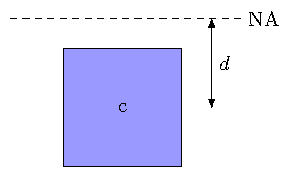
\includegraphics[width=.9\linewidth]{./pictures/parallel-axis.pdf}
\end{center}
\end{column}
\end{columns}
\end{frame}

\begin{frame}[label={sec:orged30964}]{Normal Stress in Composite Beams}
\begin{itemize}
\item From moment-curvature relationship
\end{itemize}

\[\kappa = \frac{M}{E_1 I_1 + E_2 I_2}\]

\begin{itemize}
\item From stress-curvature relationship
\end{itemize}

\[\sigma_x = - E \kappa y\]
\[\sigma_{x1} = - \frac{MyE_1}{E_1 I_1 + E_2 I_2}\]
\[\sigma_{x2} = - \frac{MyE_2}{E_1 I_1 + E_2 I_2}\]
\end{frame}

\begin{frame}[label={sec:orgbc48d3a}]{Example: Stresses in a Composite Beam}
\begin{itemize}
\item Top layer \(E\) = 200 MPa. Bottom layer \(E\) = 400 MPa. Determine
\(\sigma_{\max}\) in tension and compression.
\end{itemize}

\begin{figure}[hbtp]
  \centering
  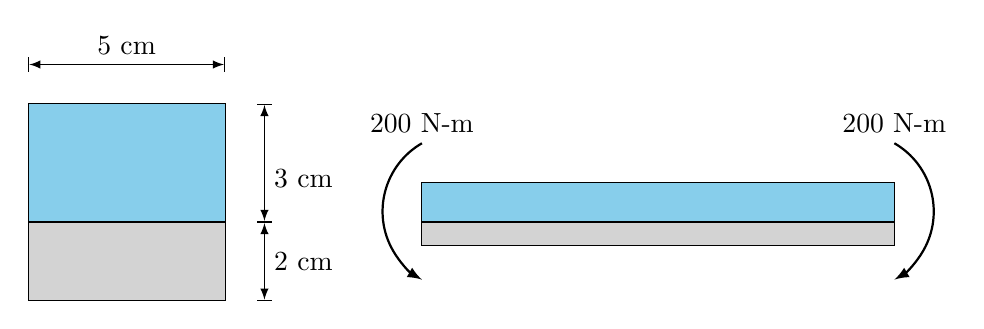
\begin{tikzpicture}[>=latex]
    \draw[fill=LightGrey] (0,0) rectangle (2.5,1);
    \draw[fill=SkyBlue] (0,1) rectangle (2.5,2.5);
    \draw[|<->|] (3,0) to (3,0.5) node[right]{2 cm} to (3,1);
    \draw[|<->|] (3,1) to (3,1.55) node[right]{3 cm} to (3,2.5);
    \draw[|<->|] (0,3) to (1.25,3) node[above]{5 cm}to (2.5, 3);
    % beam with load
    \draw[fill=LightGrey] (5,0.7) rectangle (11,1);
    \draw[fill=SkyBlue](5,1) rectangle (11,1.5);
    \draw[->, thick]  (5,2) node[above]{200 N-m} arc (120:240:1cm);
    \draw[->, thick]  (11,2) node[above]{200 N-m} arc (60:-60:1cm);
    \end{tikzpicture}
\end{figure}
\end{frame}

\begin{frame}[label={sec:orgf441077}]{Solution}
To determine stress, first we need to find neutral axis

\begin{align*}
    0 &= 200 \times {10^6}(3 \times 5)(3.5 - y_{NA}) + 400 \times {10^6}(2 \times 5)(1 - y_{NA}) \\
    0 &= 21 - 6y_{NA} + 8 - 8y_{NA} \\
    y_{NA} &= 2.07 \text{ cm}
\end{align*}
\end{frame}

\begin{frame}[label={sec:org444c8b0}]{Solution}
Calculating the area moment of inertia of each cross section, we have

\begin{align*}
    I_1 &= \frac{1}{12}(0.05)(0.03)^3 + (0.05)(0.03)(0.035 - 0.0207)^{2} \\
        &= 4.19 \times 10^{-7} \text{ m}^4 \\
    I_2 &= \frac{1}{12}(0.05)(0.02)^3 + (0.05)(0.02)(0.0207 - 0.01)^{2} \\
        &= 1.48 \times 10^{ -7} \text{ m}^4
\end{align*}
\end{frame}

\begin{frame}[label={sec:org95129f4}]{Solution}
The maximum tensile stress, occurring on the top surface of the
beam, is

\begin{align*}
  \sigma_{\max,tensile} &= \frac{MyE_1}{E_1I_1 + E_2I_2} \\
                             &= \frac{200(0.05 - 0.0207)(200 \times 10^6)}{200 \times 10^6(4.19 \times 10^{-7}) + 400 \times 10^6(1.48 \times 10^{ -7})} \\
                             &= 8.19 \text{ MPa}
\end{align*}
\end{frame}

\begin{frame}[label={sec:org87a8ef7}]{Solution}
Similarly for the maximum compressive stress at the bottom surface is

\begin{align*}
  \sigma_{\max \text{ compressive}} &= \frac{MyE_2}{E_1I_1 + E_2I_2} \\
                                 &= \frac{200(2.07 \times 10^{ - 2})(400 \times 10^6)}{200 \times 10^6(4.19 \times 10^{-7}) + 400 \times 10^6(1.48 \times 10^{-7})} \\
                                 &= 11.6 \text{ MPa}
\end{align*}
\end{frame}

\section{Bending under Inclined Loads}
\label{bending-under-inclined-loads}
\begin{frame}[label={sec:orgbd6f973}]{Bending of Beams under Inclined Loads}
\begin{itemize}
\item Normally load is applied along a symmetrical axis (\(y\) or \(z\))

\item What if it isn't?
\end{itemize}

\begin{center}
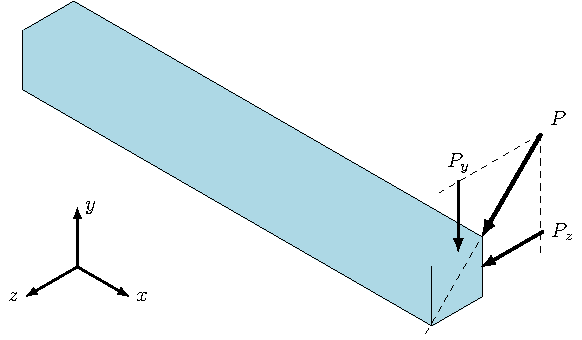
\includegraphics[width=.9\linewidth]{pictures/inclined-loads.pdf}
\end{center}
\end{frame}

\begin{frame}[label={sec:org2c3ac82}]{Superposition to the Rescue}
\begin{itemize}
\item When faced with a tough problem, break it down into smaller, easier
problems
\end{itemize}
\end{frame}

\begin{frame}[label={sec:org5a6aeab}]{Stresses from Inclined Loads}
\begin{itemize}
\item Using superposition
\end{itemize}

\[\sigma_x = \frac{M_y z}{I_y} - \frac{M_z y}{I_z}\]

\begin{itemize}
\item Neutral axis is
\end{itemize}

\[\tan \beta = \frac{y}{z} = \frac{M_y I_z}{M_z I_y}\]
\end{frame}

\section{Beam Deflection}
\label{beam-deflection}
\begin{frame}[label={sec:org3bfab5f}]{Why Do We Care about Deflection?}
\begin{itemize}
\item Stress is not always the limiting factor

\item Especially important in load-bearing structure and flexure design
\end{itemize}
\end{frame}

\begin{frame}[label={sec:orgc54f303}]{Methods of Evaluation}
\begin{itemize}
\item Direct Integration: beam curvature

\item Energy Method: strain energy
\end{itemize}
\end{frame}

\begin{frame}[label={sec:org306070d}]{Direct Integration}
\[\frac{M}{EI} = \kappa = \frac{d^2 v}{dx^2}\]

where \(v\) is the deflection function at point \(x\) along the beam
\end{frame}

\begin{frame}[label={sec:org2825d1e}]{Boundary Conditions}
\begin{itemize}
\item Indefinite integrals give constants of integration

\begin{itemize}
\item second order equations \(\rightarrow\) 2 constants
\end{itemize}

\item Need to apply knowledge about end conditions
\end{itemize}
\end{frame}

\begin{frame}[label={sec:org110effd}]{Typical End Conditions}
\begin{columns}
\begin{column}{0.5\columnwidth}
\begin{center}
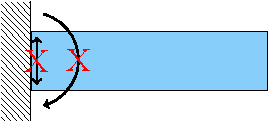
\includegraphics[width=.9\linewidth]{pictures/fixed-end.pdf}
\end{center}

\begin{center}
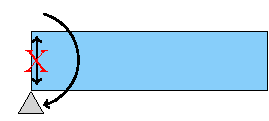
\includegraphics[width=.9\linewidth]{pictures/simple-support.pdf}
\end{center}
\end{column}

\begin{column}{0.5\columnwidth}
\begin{itemize}
\item Fixed end

\begin{itemize}
\item No deflection: \(v = 0\)

\item No rotation: \(\dfrac{dv}{dx} = 0\)
\end{itemize}

\item Simple support

\begin{itemize}
\item No deflection: \(v = 0\)

\item Free rotation:
\end{itemize}
\end{itemize}
\end{column}
\end{columns}
\end{frame}

\begin{frame}[label={sec:org03921f5}]{Example: Deflection Curve of a Cantilever Beam}
\begin{center}
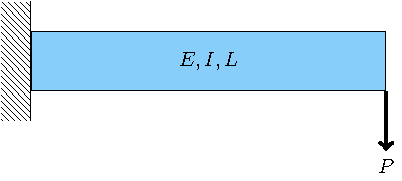
\includegraphics[width=.9\linewidth]{pictures/deflection-curve-example.pdf}
\end{center}

\begin{align*}
    \frac{d^{2}v}{dx^{2}} &= \frac{M}{EI}
\end{align*}
\end{frame}

\begin{frame}[label={sec:org0e2d6de}]{Solution}
\[M(x) =  - P(L - x)\]

Determine the deflection curve by integrating twice.

\begin{gather*}
  EI\frac{d^2v}{dx^2} = M(x) =  - P(L - x) \\
  EI\frac{dv}{dx} = \frac{P}{2}(L - x)^2 + C_1
\end{gather*}

The fixed end does not allow rotation, and so \(\frac{dv}{dx} = 0\) at
\(x = 0\).
\end{frame}

\begin{frame}[label={sec:org9c44299}]{Solution}
\begin{align*}
  C_1 &=  - \frac{PL^2}{2} \\
  EI\frac{dv}{dx} &= \frac{P}{2}(L - x)^2 - \frac{PL^2}{2} \\
  EIv &=  - \frac{P}{6}{(L - x)^3} - \frac{PL^2x}{2} + C_2
\end{align*}

At the fixed end, there is no vertical deflection, i.e. \(v = 0\) at
\(x = 0\)

\begin{align*}
  C_2 &= \frac{PL^3}{6} \\
  v &=  - \frac{P}{6EI}(L - x)^3 - \frac{PL^2x}{2EI} + \frac{PL^3}{6EI}
\end{align*}
\end{frame}

\begin{frame}[label={sec:org43ff707}]{Solution}
The maximum deflection is at the free end. Its value is

\[v(L) =  - \frac{PL^3}{2EI} + \frac{PL^3}{6EI} =  - \frac{PL^3}{3EI}\]

Note that the negative sign means the deflection is downward.
\end{frame}

\begin{frame}[label={sec:org31eef7c}]{Energy Method}
\begin{itemize}
\item Elastic deformation: way to store energy \(\rightarrow\) strain energy

\item Deflection can be derived from stored energy

\item How do we evaluate strain energy of a bent beam?
\end{itemize}
\end{frame}

\begin{frame}[label={sec:orgdb34d25}]{Strain Energy in Beam}
\begin{itemize}
\item For a small part of bent beam with length \(dx\) and bending angle
\(d\theta\)
\end{itemize}

\[d\theta = \kappa dx\]

\begin{itemize}
\item We also know from moment-curvature relationship that
\end{itemize}

\[\kappa = \frac{M}{EI}\]

\begin{itemize}
\item Assume 100\% external work to internal energy transfer
\end{itemize}

\[dW = dU = \frac{Md\theta}{2}\]

\[U = \int_0^L \frac{M^2 dx}{2EI}\]
\end{frame}

\begin{frame}[label={sec:org5dde75c}]{Castigliano's Theorem}
\begin{itemize}
\item Deflection \(v_i\) where load \(P_i\) is applied is equal to
\end{itemize}

\begin{align*}
  v_i &= \frac{\partial U}{\partial P_i} \\
      &= \int \left( \frac{M}{EI} \right) \left( \frac{\partial M}{\partial P_{i}} \right) dx
\end{align*}
\end{frame}

\begin{frame}[label={sec:orgd25dea1}]{Example: Deflection of a Cantilever Beam}
\begin{align*}
  M(x) &=  - P(L - x) \\
  \delta_i &= \int \left( \frac{M}{EI} \right)\left( \frac{\partial M}{\partial P_i} \right)dx
\end{align*}
\end{frame}

\begin{frame}[label={sec:org35c8588}]{Solution}
\begin{align*}
  \delta_{i} &= \frac{1}{EI}\int_0^L - P(L - x)[ - (L - x)]dx  \\
             &= \frac{P}{EI}\left[ L^2x - x^2L + \frac{x^3}{3} \right]_0^L \\
             &= \frac{PL^3}{3EI}
\end{align*}

\begin{itemize}
\item same answer as that of the direct integration methods

\item opposite sign though???

\item using energy method, positive means deflection is in the same
direction as the force \(\rightarrow\) down!
\end{itemize}
\end{frame}
\end{document}